\chapter{Solution}
\label{ch:Solution}
This chapter provides a solution to tackle the issue of microservice identification. As noted in the state of the art chapter \ref{ch:StateOfTheArt}, existing approaches support two initial situations: They either conduct the extraction of microservices from existing (monolithic) systems or they are based on microservice greenfield development. Both types have their advantages and disadvantages. Existing systems, for instance, provide more information about the system specification and requirements. Legacy code and log files can be used to extract data dependencies or process structures. However, shortcoming in the design of the legacy application might have an impact on the extracted information and influence the microservice extraction in a negative manner. In contrast, greenfield development is not affected by any previously committed design decisions. Nevertheless, this type has to manage the identification process with less input. \\
The solution we propose is based on pre-existing system requirements. No existing implementation is used and consequently, the presented approach is to be classified as greenfield method.\\



\section{Basic Approach}


\vspace{0.5cm}
\par
\begingroup
\leftskip=1cm
\rightskip=1cm

\noindent
\textbf{RQ1: Which is the most appropriate strategy to decompose a system into microservices? }

\endgroup
\vspace{0.5cm}




This thesis proposes a formal, graph-based microservice identification approach using clustering on control flow and data flow. The approach is  inspired by Amiri’s work on \textit{Object-aware Identification of Microservices} \cite{ObjectAwareAmiri}. 
to RQ1. Sec.5.2 suggests the improvements that form the basis of the approach
proposed by this thesis (RQ2). 


\begin{figure}[h!]
	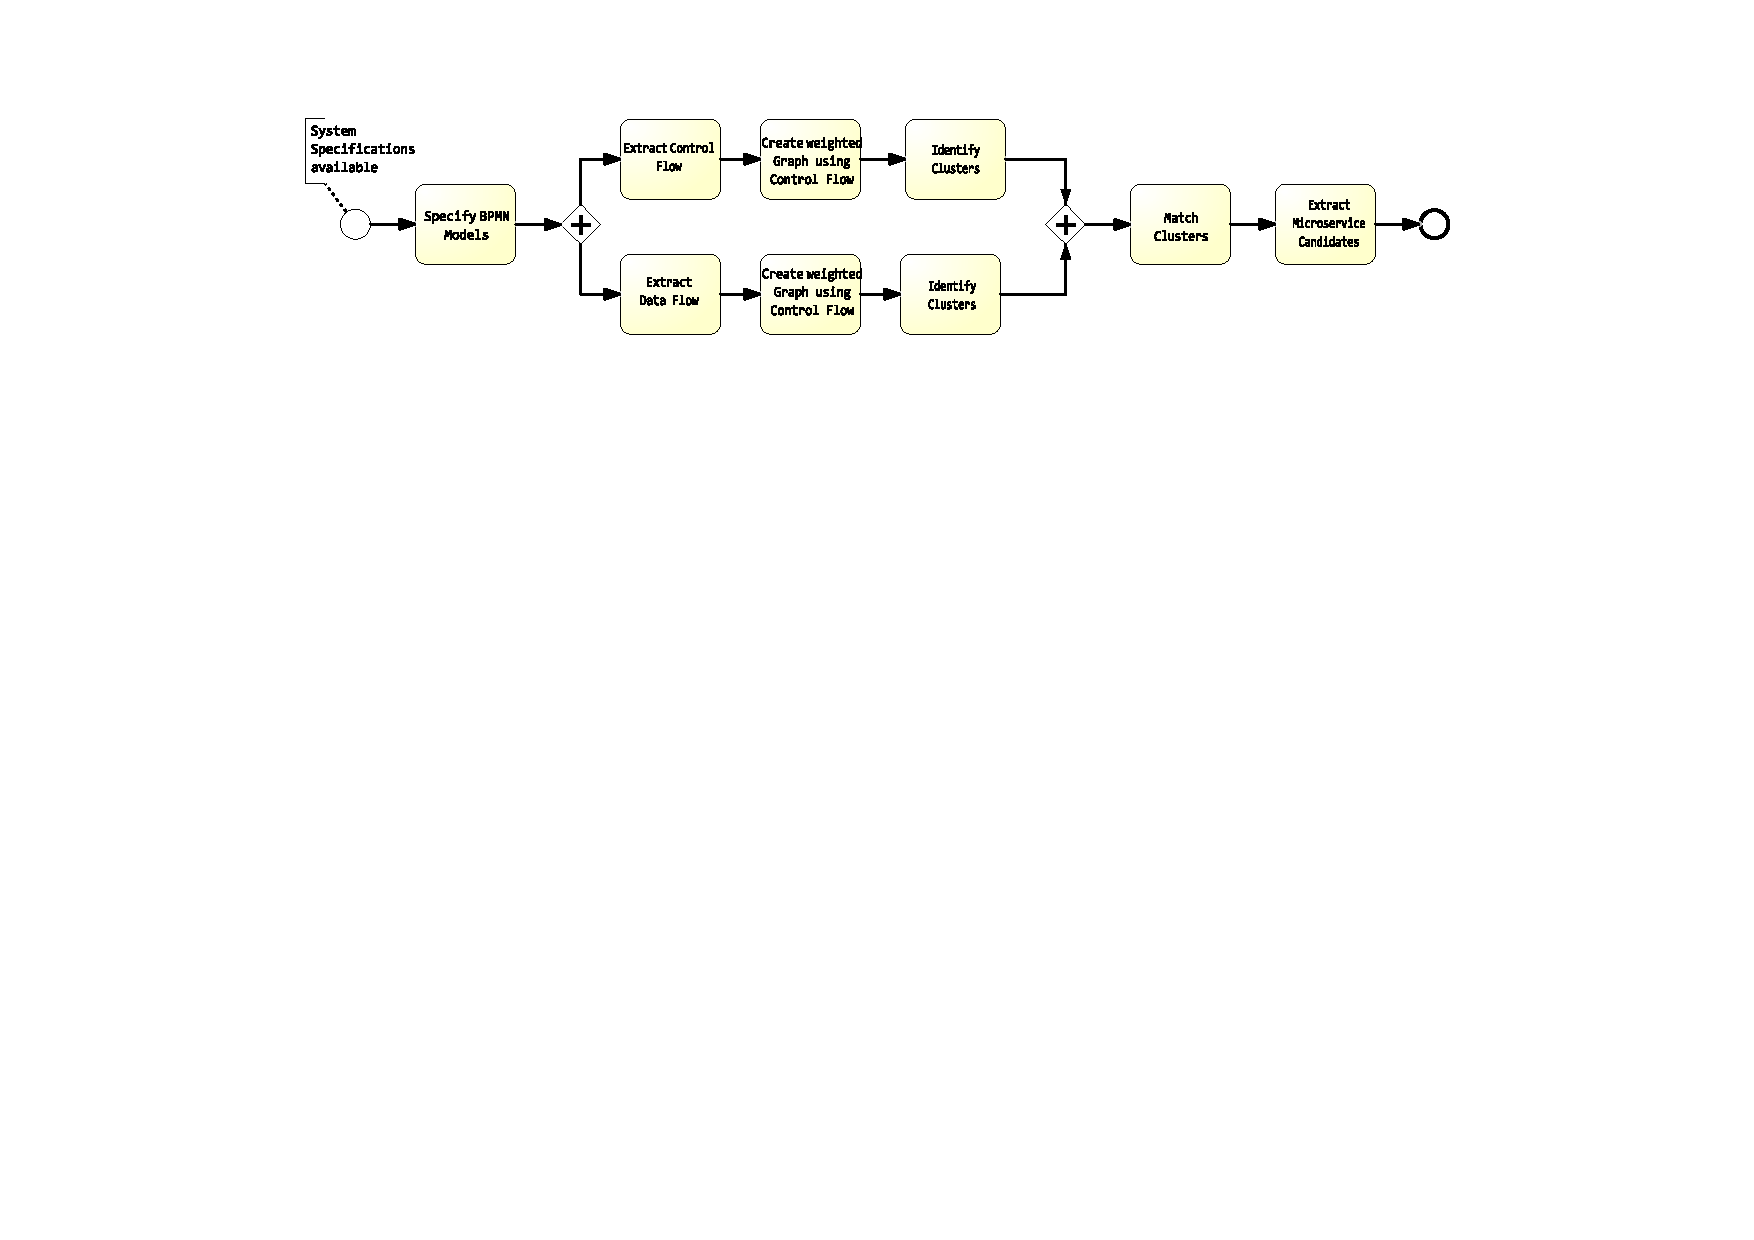
\includegraphics[width=\textwidth, trim={7.5cm 15.3cm 5.0cm 1.5cm}]{img/ThesisProcess.pdf}
	\caption{Overview of the approach}
	\label{fig:thesisProcess}
\end{figure}












\section{Distance Metric}
\begin{itemize}
	\item Determine distance between pair of Objects in BPMN (Count activities in between)
	\item Basic Idea: Data accessed more successively is more connected and belongs to same service
	\item Pro: Easy
	\item: Contra: Not really Data Flow; pair  occurs several times --> On time close, other times far away, what about average?
\end{itemize}

\section{Count Activities Metric}
\begin{itemize}
	\item Count activities that access a pair of objects in BPMN
	\item Basic Idea: Data frequently accessed together is more connected and belongs to the same service
	\item Pro: represents idea of data cohesiveness
	\item Contra: Again activities (no clean data flow) but nothing else!

\end{itemize}





